\documentclass[11pt]{article}

\usepackage{graphicx}

\begin{document}

\title{Showing that SSU is not a requirement for backward analyses}
\author{Fernando}
\maketitle

\def\SSIfy{\textsf{SSIfy}}

Our SSI intermediate representation ensures, due to the reasons that we will explain in Section~\ref{}, the Static Single Assignment property but not the Static Single Use (SSU) property.
Therefore, our program representation might have several uses of the same variable name.
In the case of a backward analysis, the sparse constraint system may have several inequations with the same left-hand side.
We illustrate this issue with Stephenson's bitwidth analysis, which combines the forward and the backward propagation of information.
Figure~\ref{fig:bitwidth}(a) contains an example of this analysis in action.
Program points $l_0$ and $l_1$ produce forward information, whereas $l_3$ produced backward information.
As an example, at program points $l_0$ we know that $a$ is upper bounded by $x$ from that point forward; similarly, at program point $l_3$ we know that $a$ cannot be greater than \texttt{v.len} from that point back.
Figure~\ref{fig:bitwidth}(d) shows the equations that we derive from this program representation.

\begin{figure}[t!]
\centering
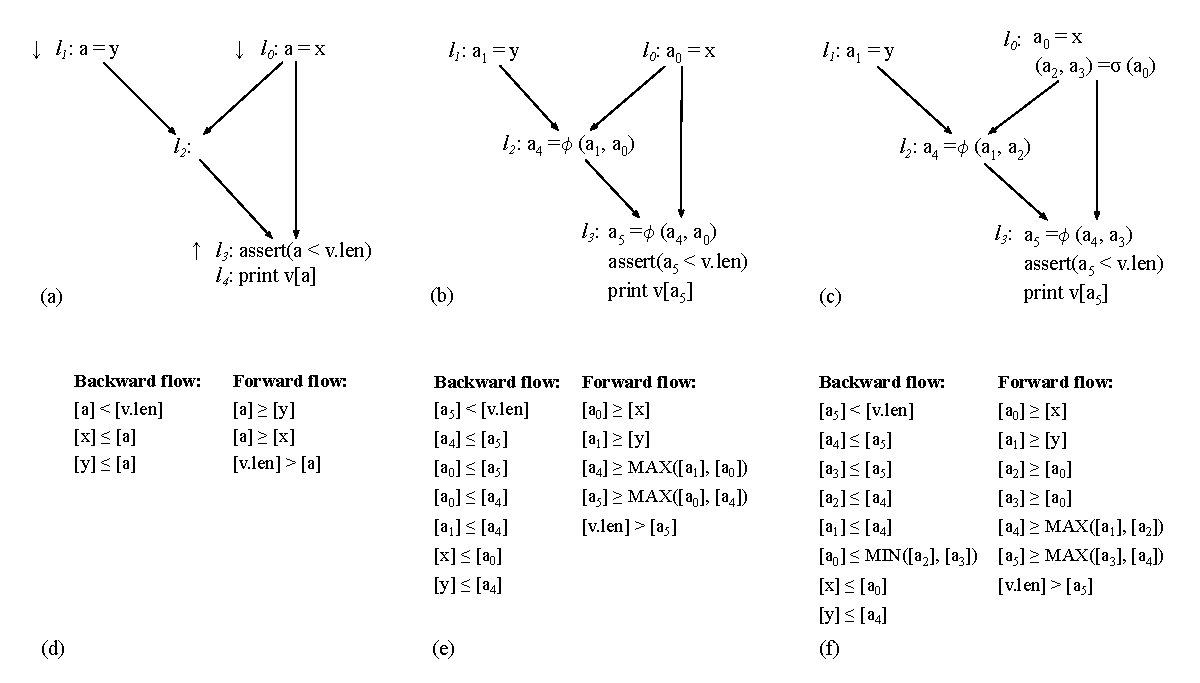
\includegraphics[width=\linewidth]{img/bitwidth}
\caption{Stephenson's bitwidth analysis.}
\label{fig:bitwidth}
\end{figure}

Figure~\ref{fig:bitwidth}(b) shows the intermediate representation that we obtain with our \SSIfy{} algorithm.
Only $l_3$ generates backward information, and its iterated dominance frontier is empty.
Therefore, we do not create any $\sigma$-function at the exit of $l_0$.
Our system of equations, shown in Figure~\ref{fig:bitwidth}(e) contains two constraints that bound the bit-size of $a_0$, e.g., $[a_0] \leq [a_4]$ and $[a_0] \leq [a_5]$.
It would still be possible to enforce the SSU property of our intermediate representation at the expenses of adding more $\phi$ and $\sigma$-functions to the program.
Figure~\ref{fig:bitwidth}(c) shows a program representation that enforces the single use property.
The $\phi$-functions at $l_2$ and $l_3$ force the creation of the $\sigma$-function at the exit of $l_0$, merging the live ranges of variables $a_2$ and $a_3$.
However, the SSU property is not necessary for every sparse analysis, and the forward-backward bitwidth analysis illustrates this point.
The two constraints $[a_0] \leq [a_4]$ and $[a_0] \leq [a_5]$ in Figure~\ref{fig:bitwidth}(e) are equivalent to $[a_0] \leq \mbox{MIN}([a_2], [a_3])$ in Figure~\ref{fig:bitwidth}(f), where MIN is the meet operator.
This equivalence hold because $[a_4]$ and $[a_5]$ contain the same backward information, as both variables propagate data coming from the same origin.

\end{document}
